\chapter{Mecánica y soporte físico del proyecto} \label{chap:Mecanica}
\chapterimage{figuras/ImagenesPortada/PortadaMecanica.jpg}
\hrule
\vspace{3mm}

Una vez vistas algunas ideas previas generales que deberá tener el prototipo diseñado este capítulo entra de lleno en la descripción de la solución mecánica obtenida así como una comparación con ideas previas.

\section{Visión general y materiales estructurales} \label{sec:Mecanica:vision_general}

    Antes de empezar a repasar los detalles concretos es necesario establecer unos convencionalismos respecto al uso de nomenclatura.
    \\

    Como se ha descrito en el capítulo \ref{chap:Punto_partida} el movimiento de las articulaciones encargadas de posicionar el extremo del robot se transmitirá de forma mecánica desde los motores hasta la propia articulación. Aunque no viene impuesto por ningún requisito funcional, se ha optado por fijar los tres primeros grados de libertad de tipo rotacional. En la figura \ref{fig:Mecanica:convenciones_generales} se puede ver un diagrama esquematizado de un brazo robótico con tres grados de libertad rotacionales. A partir de ahora se hará referencia a los tres primeros grados de libertad como los \ingles{GDL} o articulaciones de posición.
    \\

    En la imagen se puede ver como serán nombradas las primeras tres articulaciones también se debe aclarar la nomenclatura a utilizar sobre los elementos que unen dichas articulaciones. Serán llamados indistintamente eslabones o barras estando numerando desde la barra cero, que conecta el suelo con el primer grado de libertad, en adelante.

    \begin{figure}[H]
        \centering
        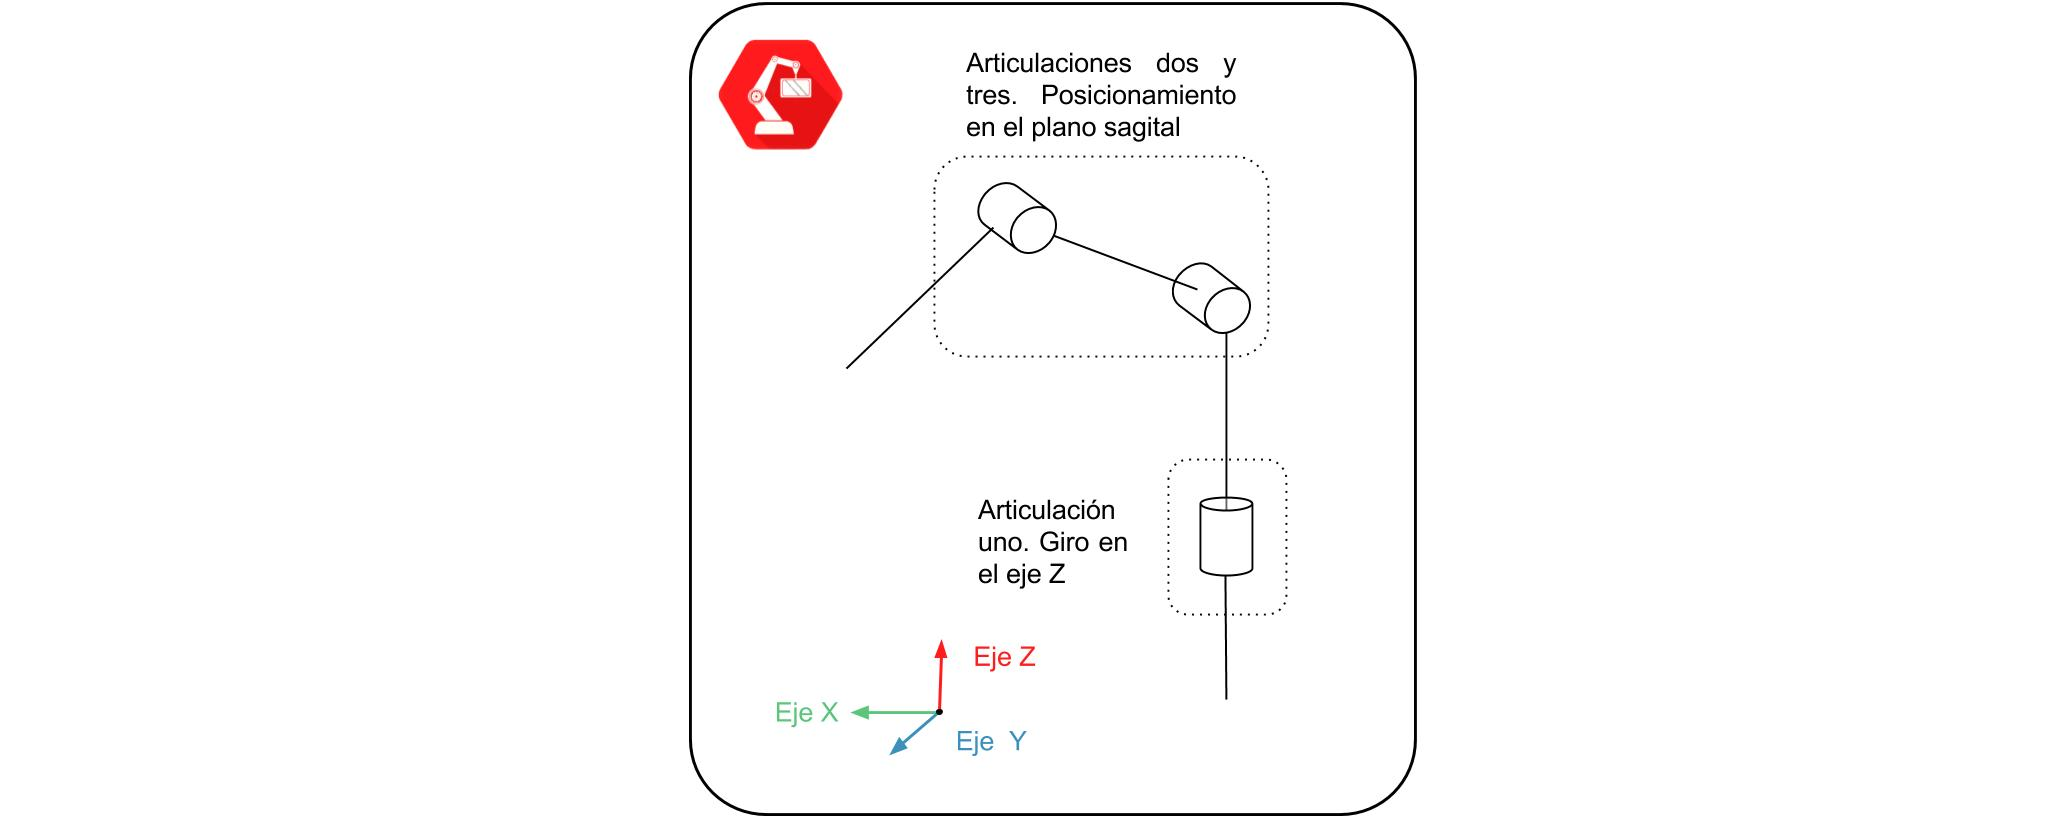
\includegraphics[width=\textwidth]{figuras/Imagenes_Mecanica/modelo_esquematico.jpg}
        \caption{Modelo de los grados de libertad de posición. Convencionalismos tomados}
        \label{fig:Mecanica:convenciones_generales}
        \immagesource{Autor}
    \end{figure}

    Como se ha comentado en secciones anteriores el brazo debe ser capaz de orientar la tablet de forma que ésta sea capaz de \textit{ver} y seguir los ojos del paciente. Aunque el brazo podría anclarse a diferentes estructuras de ahora en adelante se centra la justificación y desarrollo en el caso de uso sobre una camilla. Este caso es el que requiere mayor longitud de trabajo de forma que las dimensiones del brazo deberán permitirle abarcar de un lado a otro de la camilla.
    \\

    Este espacio de trabajo definido, que deberá abarcar aproximadamente $90cm$ (la mayoría de camas y camillas tienen esta medida), implica unas dimensiones de los eslabones del brazo considerables. Como se ha visto en capítulos anteriores el peso del prototipo es un factor importante tanto para la seguridad del usuario como para que pueda ser desplazado por unos motores de bajo par.
    \\

    La transmisión mecánica del movimiento debe optimizarse para ser capaz de mover el brazo; este trabajo se verá simplificado a su vez aligerando, cuando sea posible, la estructura del mismo. Como material estructural base se han elegido perfiles de aluminio de sección cuadrada (se describen en detalle en el capítulo \completar junto con el resto de materiales). Estos perfiles presentan una alta resistencia y capacidad de carga a la vez que un peso reducido.
    \\

    El material estructural definido se complementa con otra serie de piezas diseñadas específicamente para este proyecto (se puede ver el anexo \ref{app:listadoPiezas} para ver estas piezas). En este caso, por su versatilidad se utilizarán piezas modeladas digitalmente e Impresas en 3D posteriormente. De igual manera parte del diseño se apoya en piezas de metacrilato cortado con láser.
    \\

    Aunque el peso del brazo completo se estima será reducido, la transmisión mediante cuerdas debe ser completamente fiable. Debido a las dimensiones con las que se trabaja se ve inviable el uso de cadenas o cuerdas de gran grosor; es por eso que se ha optado por utilizar hilo de \ingles{kevlar} de un milímetro de grosor.
    \\

    Aunque supone anticipar parte del desarrollo que se verá a continuación, a modo de lista se pueden resumir los materiales necesarios a nivel constructivo del proyecto en:
    \begin{itemize}
        \item Barras de aluminio de sección cuadrada de 1/2"x1m (lado de la sección x longitud).
        \item Rodamientos de bolas de 4mm x 13mm (diámetro interior X diámetro exterior)
        \item Rodamientos de bolas de 3mm x 10mm (diámetro interior X diámetro exterior)
        \item Rodamiento axial de 37.5mm x 52mm (diámetro interior X diámetro exterior)
        \item Barras de acero macizo cilíndricas de 4mm de diámetro
        \item Barras de acero macizo cilíndricas de 3mm de diámetro
        \item Piezas impresas en impresora 3D. (Lista detallada en el Anexo \ref{app:listadoPiezas})
        \item Piezas de metacrilato cortadas con láser. (Lista detallada en el Anexo \ref{app:listadoPiezas})
        \item Tornillería: tornillos y tuercas de diferentes métricas.
        \item Hilo de kevlar.
        \item Poleas de acetal de 4.9mm x 21.8mm (diámetro interior X diámetro exterior).
        \item Soporte de sombrilla. La base sobre la que se apoye el brazo debe ser capaz de soportarlo en una posición de trabajo en todo momento. Para no fijar ni imponer ningún tipo de anclaje (a superficie plana, anclaje a una camilla, etc) se ha optado por esta solución para el desarrollo del prototipo.
    \end{itemize}

    En el capítulo \ref{chap:Gestion}, concretamente en la tabla \ref{tab:presupuesto}, están reflejados los detalles técnicos de estos materiales así como las referencias de compra, cantidades necesarias y precios.

\section{Filosofía y justificación de diseño} \label{sec:Mecanica:filosofia_diseno}

    Tal y como se ha adelantado en el capítulo introductorio el software empleado para modelar el brazo robótico es Autodesk Inventor. Este programa es especialmente potente para modelado paramétrico; esto significa que permite definir una serie de parámetros que serán utilizados para definir las medidas de los bocetos. Un diseño bien modelado parametricamente permite mucha flexibilidad a la hora de modificar ciertas medidas como pueden ser agujeros para tornillería, ejes u holguras.
    \\

    El modelado de todas las piezas ha seguido esta filosofía de parametrización y dependencia entre las piezas de forma que el diseño sea lo más flexible posible en cuanto a modificación de medidas. En la figura \ref{fig:Mecanica:diseno_parametrico} se puede ver a modo de ejemplo parte de la lista de parámetros definida.

    \begin{figure}[H]
        \centering
        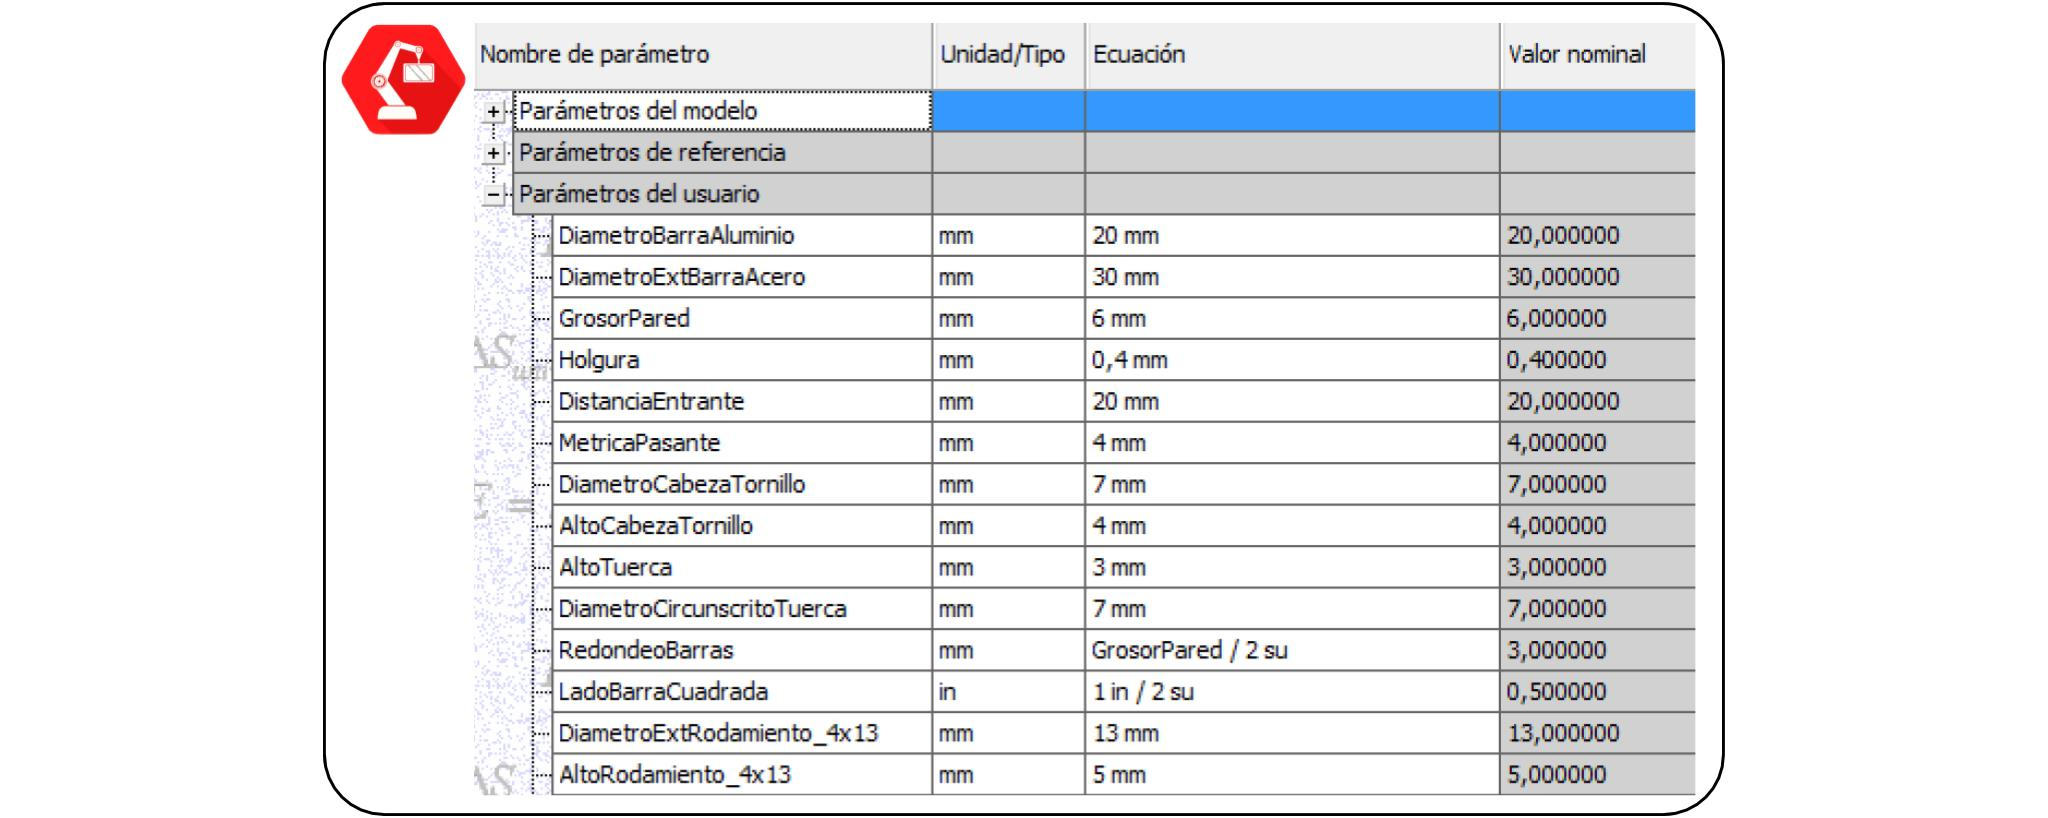
\includegraphics[width=\textwidth]{figuras/Imagenes_Mecanica/diseno_parametrico.jpg}
        \caption{Ejemplo de parámetros definidos en Inventor}
        \label{fig:Mecanica:diseno_parametrico}
        \immagesource{Autor}
    \end{figure}

\subsection{Realidad de las formas}
    Cualquier diseño de producto, incluso desde un punto de vista más técnico incluye a su vez consideraciones sobre el diseño estético del mismo. Para este proyecto se ha intentado respetar la verdad de las formas predominantes tanto a nivel estructural como en el entorno de trabajo.
    \\

    Como ya se ha visto, la base estructural del prototipo está conformada por barras de aluminio de sección cuadrada. Unido a la predominancia de formas rectangulares y/o cuadradas en una habitación de hospital (figura \ref{fig:Mecanica:verdad_formas}) se ha optado por un diseño basado en prismas rectangulares, con un aspecto más \ingles{retro}.
    \\

    A nivel bibliográfico y del estado del arte estudiado se puede observar una tendencia a formas más suavizadas en muchos de los casos. En este proyecto se busca un contraste entre las formas que caracterizan al ser humano, más suavizadas y con geometrías complejas, en contraposición con las formas que definen el prototipo, formas geométricas y angulares.

    \begin{figure}[H]
        \centering
        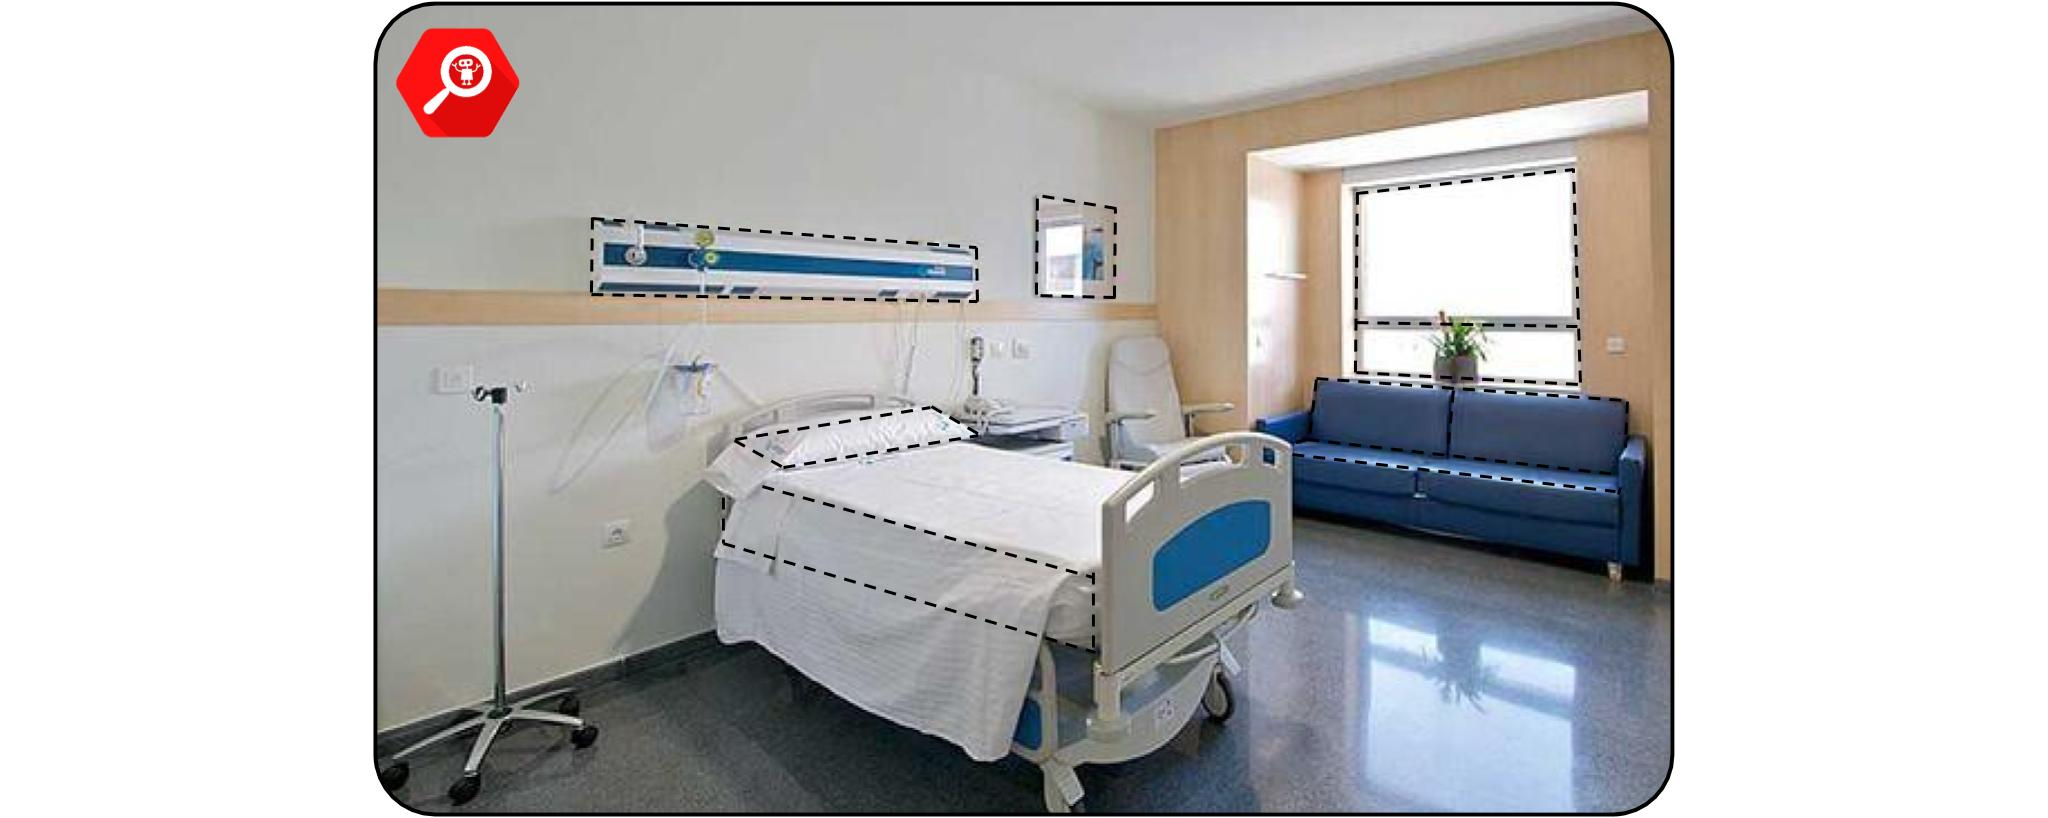
\includegraphics[width=\textwidth]{figuras/Imagenes_Mecanica/verdad_de_formas.jpg}
        \caption{Predominancia de formas rectangulares en el entorno de trabajo}
        \label{fig:Mecanica:verdad_formas}
        \immagesource{Imagen de consalud.es, editada posteriormente por el Autor}
    \end{figure}

\section{Articulación uno. Giro en el eje Z} \label{sec:Mecanica:articulacion_uno}

    Volviendo sobre el diseño mecánico, la primera articulación que se encuentra subiendo desde la base es la encargada de girar todo el robot en el eje Z.

    Esta articulación está actuada por un Servo motor (descrito en detalle en el Capítulo \ref{chap:Electronica}. Como se ha anticipado el movimiento de este servo se transmite a través de un juego de ruedas que, solidarias a la parte superior (parte móvil), y por rozamiento, transmiten el movimiento de giro con respecto a la parte inferior (parte fija o base).
    \\

    Una de las ruedas gira solidaria al servo motor, haciendo contacto firme con la rueda a continuación (rueda transmisora). Ésta será la encargada de transmitir el par sobre la superficie sobre la que apoya. El peso del brazo sobre dicho apoyo es suficiente como para asegurar que en condiciones normales de funcionamiento la articulación gire con normalidad; en caso de chocar contra aun usuario la fuerza será mayor y la rueda transmisora deslizará sobre la superficie inferior evitando daños al usuario.
	\\
	En la figura \ref{fig:Mecanica:giro_z} se puede ver en detalle el montaje de dicha estructura. Las piezas que aparecen en la imagen se pueden encontrar en mayor detalle descritas en el Anexo \ref{app:listadoPiezas}.

	\begin{figure}[H]
		\centering
		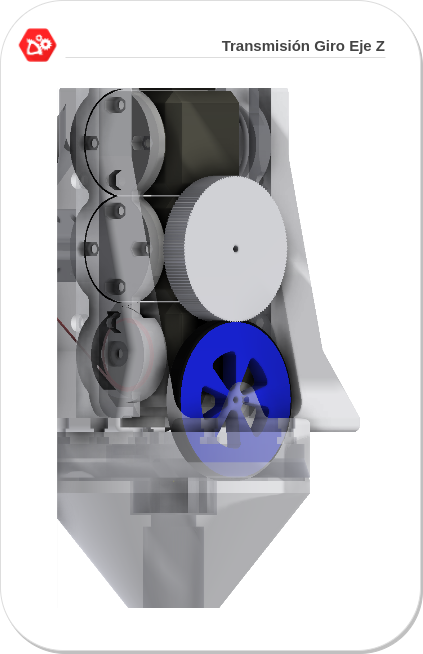
\includegraphics[width=0.5\textwidth]{figuras/Imagenes_Mecanica/RuedasGiroZ.png}
		\caption{Montaje de la transmisión del movimiento del servo a la articulación encargada de girar en Z \completarCon{cambiar por foto buena}}
		\label{fig:Mecanica:giro_z}
		\immagesource{Autor}
	\end{figure}

	Una vez vista la transmisión del movimiento queda otro punto importante, el apoyo del peso del brazo sobre la articulación. Referente a este punto se han explorado dos líneas del desarrollo posibles:
    \begin{itemize}
        \item Apoyo sobre ruedas: Además de la rueda transmisora se fijan a la parte móvil de la articulación una serie de ruedas sobre las que apoyará el brazo. Inicialmente puede parecer que el apoyo será más estable cuantos más puntos tenga; desde el punto de vista práctico incluir apoyos redundantes genera más problemas a la larga. Tres puntos son suficientes para definir un plano y es el número de ruedas óptimo a utilizar: dos ruedas de apoyo más la rueda de transmisión. Se puede ver en detalle como queda el montaje en la figura \ref{fig:Mecanica:apoyo_ruedas}. Como se puede ver el diseño incluye unas piezas en metacrilato, en concreto la pieza solidaria a la parte fija del robot cuenta con una la superficie ranurada (realizado a modo de grabado con la máquina de corte láser) para aumentar el rozamiento con la rueda de transmisión. Las ruedas de apoyo están ubicadas a la misma distancia del eje de giro que la rueda transmisora.
        \item Apoyo sobre rodamiento: El apoyo se realiza sobre un rodamiento axial; quedando junto a ambas piezas, superior e inferior, incrustados entre si. Sobre este punto se apoya el peso del brazo y el encaje entre las piezas impide que el eje del brazo se mueva de la vertical. El uso de un rodamiento implica reducir la distancia sobre la que se apoya el peso, aunque permite fijar por ambos lados las piezas al rodamiento de forma más firme. Finalmente ésta es la opción adoptada para el brazo robótico por aportar una mayor solidez y estabilidad al aportar puto de apoyo continuo en los $360^o$ al rededor del eje.
    \end{itemize}

    \begin{minipage}{0.47\textwidth}
        \begin{figure}[H]
            \centering
            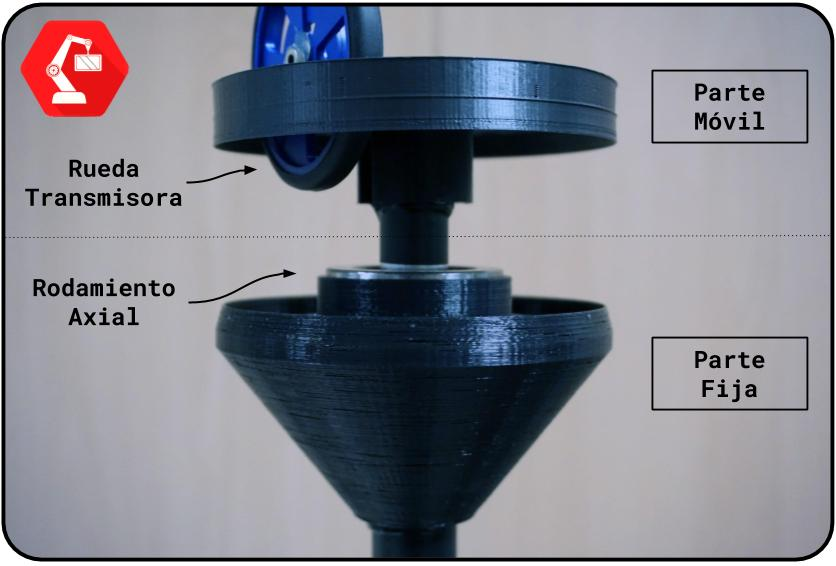
\includegraphics[width=\textwidth]{figuras/Imagenes_Mecanica/foto_brazo_12.jpg}
            \caption{Apoyo basado en un rodamiento Axial}
            \label{fig:Mecanica:apoyo_rodamiento_axial}
            \immagesource{Autor}
        \end{figure}
    \end{minipage}
    \begin{minipage}{0.47\textwidth}\raggedright
        \begin{figure}[H]
            \centering
            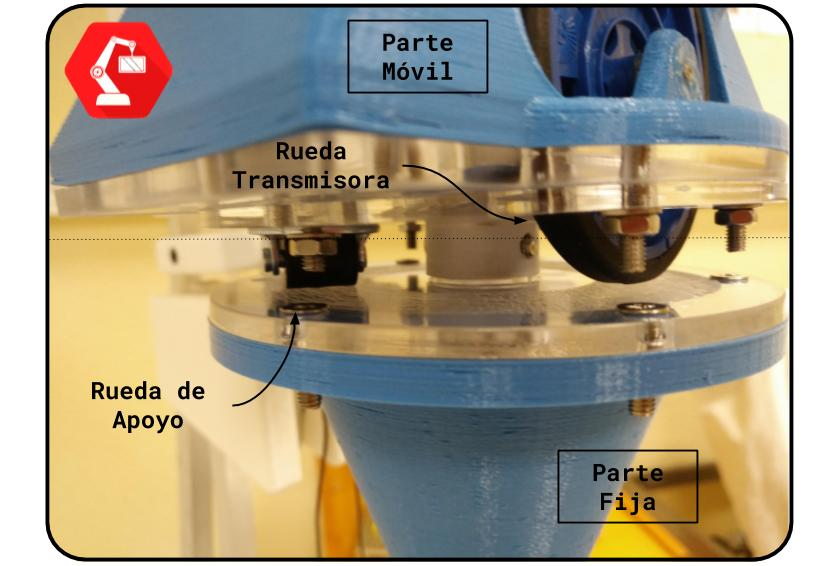
\includegraphics[width=\textwidth]{figuras/Imagenes_Mecanica/foto_brazo_anterior_1.jpg}
            \caption{Apoyo basado en ruedas}
            \label{fig:Mecanica:apoyo_ruedas}
            \immagesource{Autor}
        \end{figure}
    \end{minipage}

    Además del tipo de apoyo se debe valorar en qué lado se sitúa la rueda de transmisión. Anticipando siguientes apartados la estructura del brazo sobresale por uno de los lados. En caso de ubicar la rueda motriz en el lado opuesto la carga dificulta el apoyo de la misma. En el caso de apoyo con ruedas además se apoya todo el peso sobre un voladizo, la distancia entre las dos ruedas de apoyo contrarias a la rueda de transmisión. Aunque en el caso del apoyo mediante rodamiento axial este efecto se suaviza, ya no apoya sobre un voladizo, el diseño final aprovecha la carga del brazo para asegurar el apoyo de la rueda de transmisión. En caso de que la explicación textual no sea suficientemente explicativa, se puede ver una representación gráfica de las diferentes situaciones en la figura \ref{fig:Mecanica:apoyo_carga}.

    \begin{figure}[H]
        \centering
        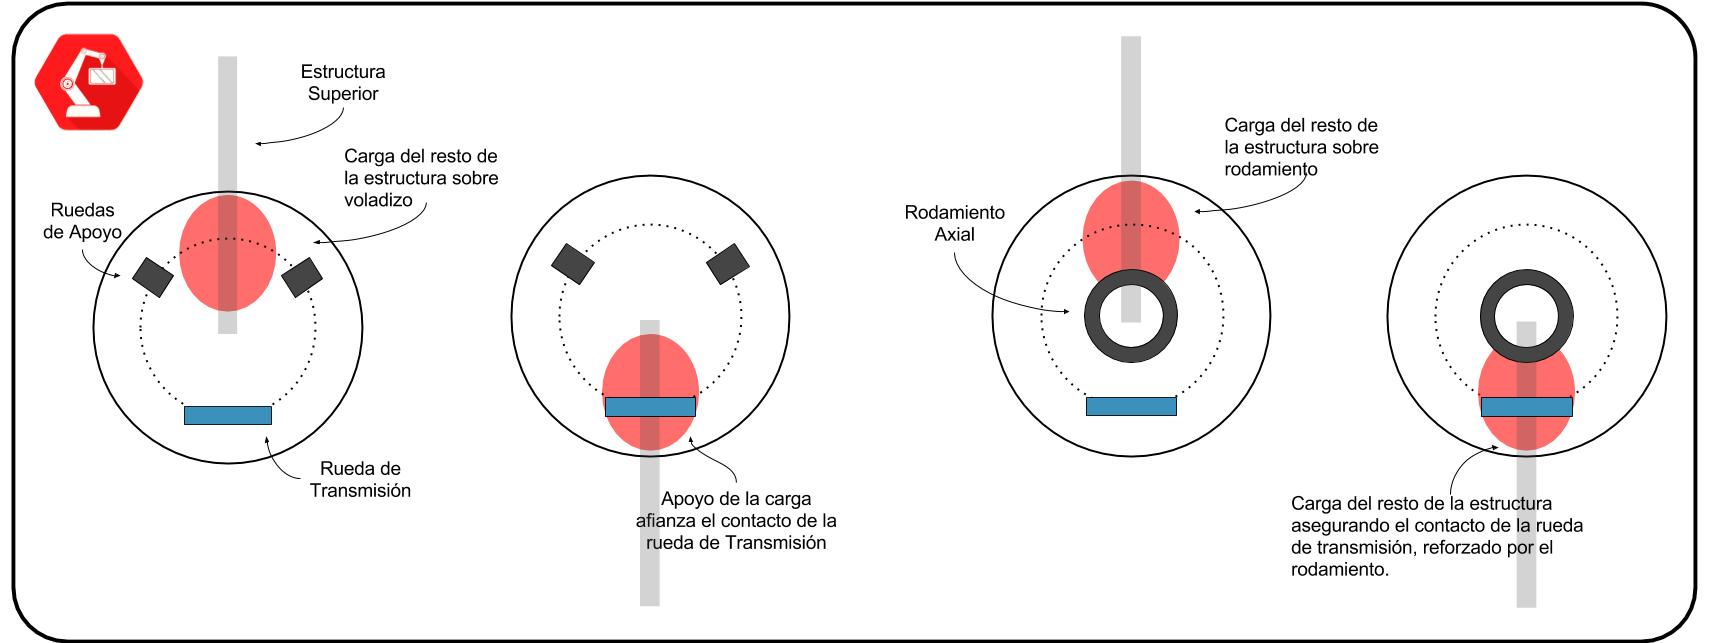
\includegraphics[width=\textwidth]{figuras/Imagenes_Mecanica/comparacion_apoyos.jpg}
        \caption{Comparación de como afecta el punto de apoyo de la carga superior sobre los diferentes apoyos}
        \label{fig:Mecanica:apoyo_carga}
        \immagesource{Autor}
    \end{figure}

    Toda esta estructura va montada sobre una base que ejerce de contrapeso para evitar que el eje central del brazo (eje Z) se incline. Como se ha visto anteriormente para esta base se ha adaptado un contrapeso de sombrilla sobre el que encaja el brazo. Este apoyo podría modificarse e incluso adaptar una fijación a otra superficie en caso de montar el brazo en otro entorno.

    \completarCon{¿Debería añadir una imagen con el pie y esta articulación o ya es pasarse de imágenes? La tengho hecha realmente así que...}

\section{Articulaciones dos y tres. Posicionamiento en el plano sagital} \label{sec:Mecanica:articulacion_dostres}

    Las articulaciones dos y tres, representadas de forma esquemática en la figura \ref{fig:Mecanica:convenciones_generales} son las encargadas de posicionar el robot en el plano sagital del robot. Este plano girará al rededor del eje Z gracias a la articulación primera, vista en la sección anterior. Como se ha anticipado en el capítulo \ref{chap:Punto_partida} estas dos articulaciones están conformadas por dos mecanismos de cuatro barras acopladas en serie.
    \\

    La figura \ref{fig:PuntoPartida:maquetas} del capítulo \ref{chap:Punto_partida} ya anticipaba diferentes métodos de acople entre los mecanismos , cada uno presentando sus virtudes y desventajas.
    \\

	\completarCon{Tenía pensado incluir el modo "grua" que provamos al inicio en la descripción, pero puede que alargue y líe el capítulo más}
	
	La situación final elegida basa por presentar ambos mecanismos las mismas dimensiones siendo sus barras iguales dos a dos. Una cadena de eslabones configurada de esta manera, aunque alarga la necesidad de transmitir el movimiento hasta cada eje de giro, tiene la particularidad de que mantiene la orientación del extremo del brazo siempre paralela a la de la barra de acople y en este caso, al eje Z. En la figura \ref{fig:Mecanica:4_bar_mecanism} se pueden ver los puntos sobre los que se actúan ambas articulaciones. Concretamente se ha diseñado de forma que tanto el extremo como la barra acopladora se mantienen siempre perpendiculares al plano del suelo como se puede apreciar en la figura \ref{fig:Mecanica:movimiento}.
    \\

    \begin{figure}[H]
    	\centering
    	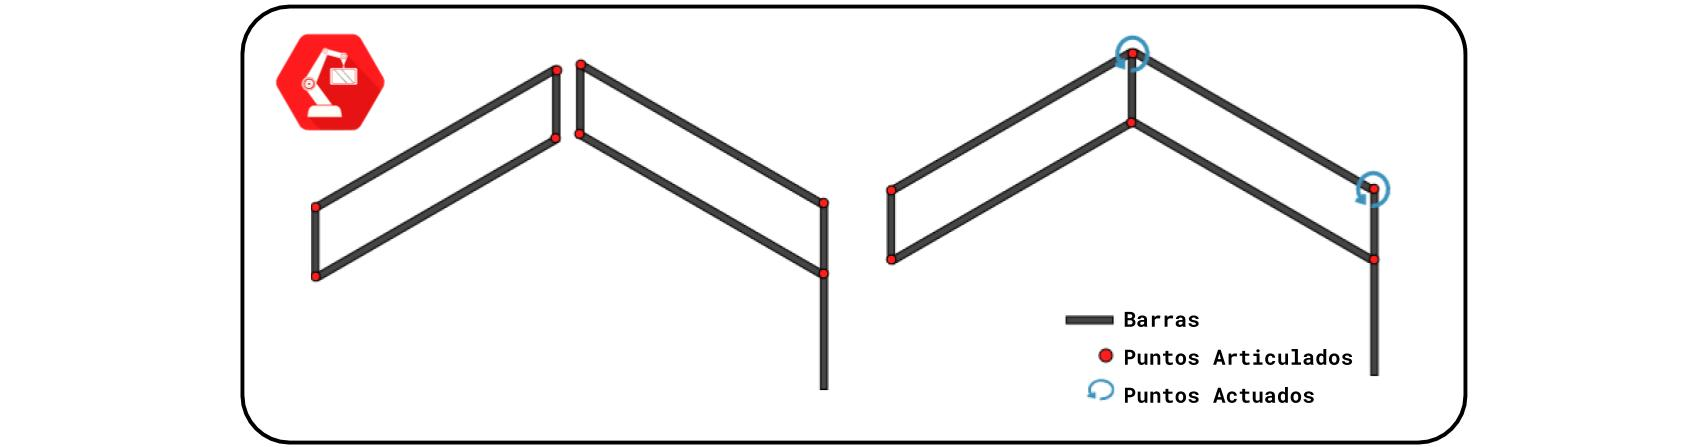
\includegraphics[width=\textwidth]{figuras/Imagenes_Mecanica/mecanismos_4_barras.jpg}
    	\caption{Esquema de las articulaciones dos y tres. Estructura de unión lineal}
    	\label{fig:Mecanica:4_bar_mecanism}
    	\immagesource{Autor}
    \end{figure}
    
    
    \begin{figure}[H]
       	\centering
       	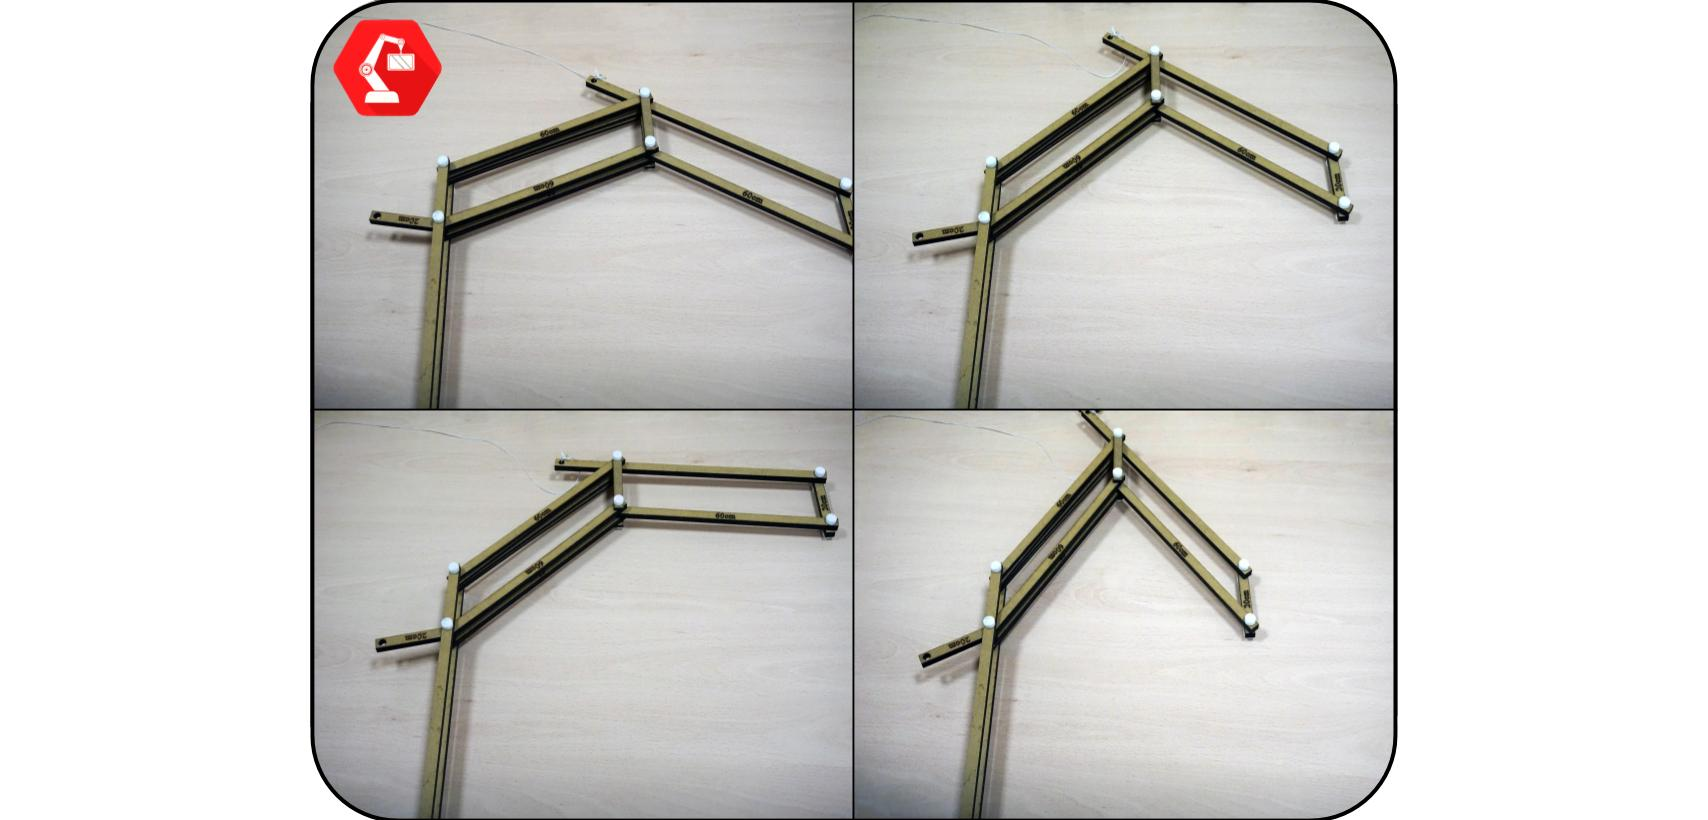
\includegraphics[width=\textwidth]{figuras/Imagenes_Mecanica/movimiento_maqueta.jpg}
       	\caption{Diferentes posiciones articulares manteniendo la barra acopladora y el extremo perpendiculares}
       	\label{fig:Mecanica:movimiento}
       	\immagesource{Autor}
    \end{figure}

    Se ha adelantado en el capítulo \ref{chap:Punto_partida} la importancia de compensar el peso. En \cite{Rahman_asimple} se puede encontrar una demostración matemática de como se puede compensar, mediante el uso de muelles, el peso del los eslabones. Ambas estructuras expuestas permiten este tipo de compensación de la carga. Finalmente se ha optado por la segunda opción (acoplamiento lineal) ya que mantiene la orientación del extremo siempre constante y perpendicular al plano del suelo. Esta característica resulta muy útil ya que simplifica el análisis matemático y posterior control del brazo robótico en gran medida.
    \\
    
    En versiones anteriores se ha probado con diferentes tipos de acoplamiento, en la figura \ref{fig:Mecanica:geometria_acopladora} se puede ver como afecta esta pieza a la orientación del extremo en base a maquetas preparadas.
    
    \begin{figure}[H]
    	\centering
    	
\includegraphics[width=\textwidth]{figuras/Imagenes_Mecanica/transicion_maqueta.jpg}
    	\caption{Diferentes geometrías de la barra acopladora}
    	\label{fig:Mecanica:geometria_acopladora}
    	\immagesource{Autor}
    \end{figure}

    Aunque en el esquema sobre el papel cuadre bien un acoplamiento lineal, en la realidad esto supone el apilamiento de muchos componentes sobre la misma barra. En ese caso la estructura resultante va engrosando y alejándose del plano sagital, lo que a futuro puede provocar fuerzas transversales indeseadas. 
    
    Para el montaje este acoplamiento lineal se ha separado formando una geometría de tipo paralelogramo (en línea con la representación de la figura \ref{fig:Mecanica:geometria_acopladora}), concretamente romboide. Está conformado por una base de metacrilato con piezas de apoyo impresas en plástico que atrapan, a modo de \textit{sándwich}, las barras estructurales de aluminio.

    \begin{figure}[H]
        \centering
        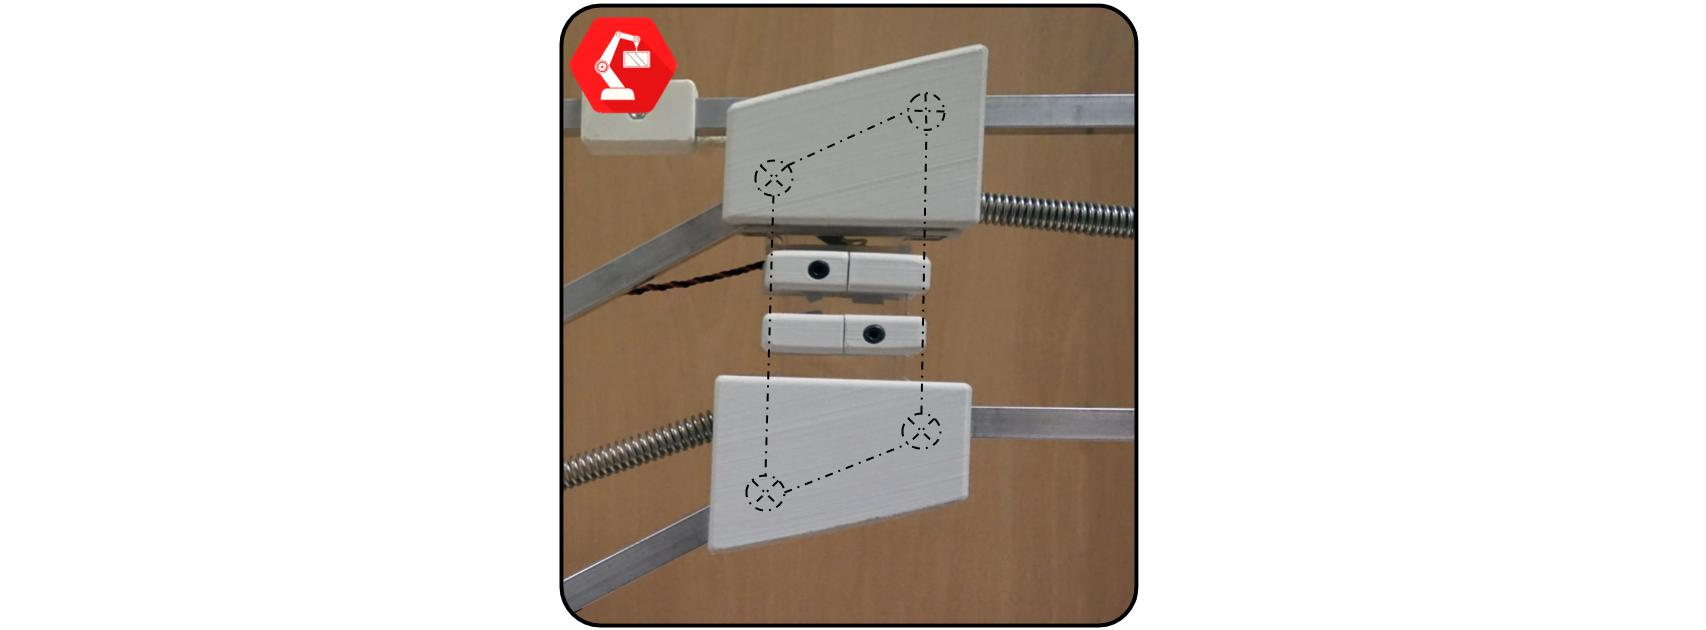
\includegraphics[width=\textwidth]{figuras/Imagenes_Mecanica/acoplamiento_romboide.jpg}
        \caption{Imagen del acoplamiento \textit{romboide}}
        \label{fig:Mecanica:acoplamiento_romboide}
        \immagesource{Autor}
    \end{figure}

    Volviendo sobre la compensación del peso del robot, se ha seguido una estrategia similar aunque simplificada a la planteada por \cite{Rahman_asimple}. El propósito de los muelles, uno para cada mecanismo, es el de compensar el peso de toda la estructura del brazo de forma que, en vacío, el brazo tenderá a elevarse. Será el peso de la \ingles{tablet} una vez se acople el culpable del funcionamiento del brazo tal y como se ha planteado: el manipulador asciende gracias al par aportado por los servomotores; y desciende por gravedad.
    \\

    En la figura \ref{brazo_con_muelles} se puede ver el montaje de las barras con los muelles que, de forma cruzada, se oponen al peso de la estructura. En esta imagen se anticipa algunos conceptos y servirá como mapa general para localizar diferentes componentes del brazo robótico sobre los que se focalizará a continuación.

    \begin{figure}[H]
        \centering
        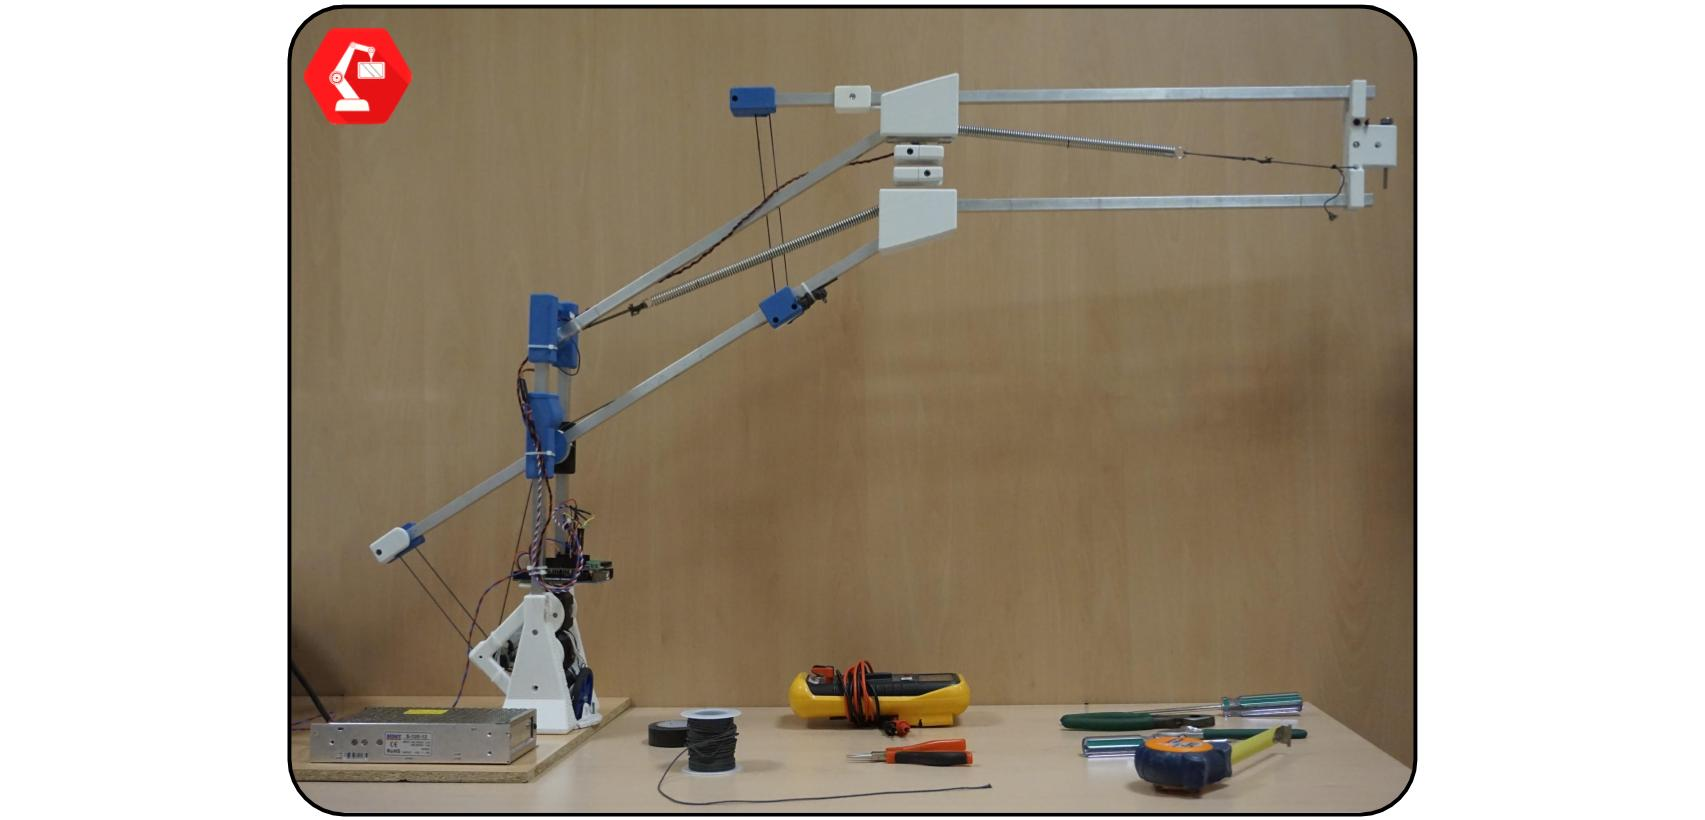
\includegraphics[width=\textwidth]{figuras/Imagenes_Mecanica/foto_brazo_10.jpg}
        \caption{Vista genérica de los grados de libertad dos y tres}
        \label{fig:Mecanica:brazo_con_muelles}
        \immagesource{Autor}
    \end{figure}


    La transmisión del movimiento para estos dos grados de libertad se ha realizado a través de hilos que van desde los servomotores hasta la articulación. Esos hilos están configurados de forma que no retornan hasta la polea de salida, polea acoplada al giro del motor. La transmisión está preparada para tirar de la carga de forma activa cuando se quiere subir la muñeca del robot, soltando cuerda en el caso contrario para dejarlo descender poco a poco.
	\\

    En el caso de ambas articulaciones la carga recibida por el motor ha sido reducida a través de elementos mecánicos sencillos. El enganche para ambas articulaciones hace uso de la misma filosofía. Se ha alejado el punto de actuación del eje de giro para conseguir una palanca sobre la que se actúa maximizando así la fuerza realizada por el servo.
    \\

    A su vez se ha aprovechado el concepto de \textit{polipasto} ampliamente utilizado en actividades de trabajo vertical en las que sea necesario elevar cargas demasiado pesadas para ser manipuladas por una persona. Descritas en detalle por \cite{granvertical} basan su funcionamiento en combinar el uso de poleas fijas y móviles de forma que, el cable que las recorre, queda conectado a un punto fijo. De esta manera se reduce la fuerza necesaria para desplazar la carga, que estará acoplada a una de las poleas móviles.

    \begin{minipage}{0.30\textwidth}
        \begin{figure}[H]
            \centering
            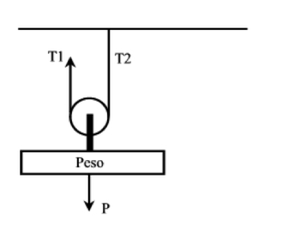
\includegraphics[width=\textwidth]{figuras/Imagenes_Mecanica/pmovil.png}
            \caption{Polea Móvil}
            \label{fig:Mecanica:pmovil}
            \immagesource{\cite{granvertical}}
        \end{figure}
    \end{minipage}
    \begin{minipage}{0.60\textwidth}\raggedright

        La figura \ref{fig:Mecanica:pmovil} representa una polea móvil de forma similar a como se ha aplicado en el proyecto. Como puntualiza \cite{granvertical} siempre y cuando las cuerdas se mantengan paralelas se obtiene una reducción de la fuerza necesaria para mover la carga \textbf{P} del 50\%. Esta sencilla demostración se puede ver en \ref{eq:Mecanica:polipasto}, que se deduce de un punto de equilibrio estático:
        \begin{equation}
            \label{eq:Mecanica:polipasto}
            P = T1 + T2 ; T1 = T2 ; T1 = frac{P}{2}
        \end{equation}
        Es importante remarcar que ésta relación es una relación matemática; en la práctica, como bien apunta \cite{granvertical}, el rozamiento supondrá pérdida del rendimiento. En función de la calidad de los rodamientos de la polea se obtendrán rendimientos de entre el 70\% y el 97\%.
    \end{minipage}

    Volviendo sobre el diseño del brazo se ha diseñado de forma que en todo momento ambas cuerdas se mantendrán paralelas; además las poleas están montadas sobre dos rodamientos que aseguran un mayor rendimiento de la amplificación mecánica. Se pueden ver ambos montajes (palanca y polipasto) en las figuras \ref{fig:Mecanica:columpio_art_uno} y \ref{fig:Mecanica:columpio_art_dos} el montaje de estos \textit{columpios} para ambas articulaciones.

    \begin{minipage}{0.41\textwidth}
        \begin{figure}[H]
            \centering
            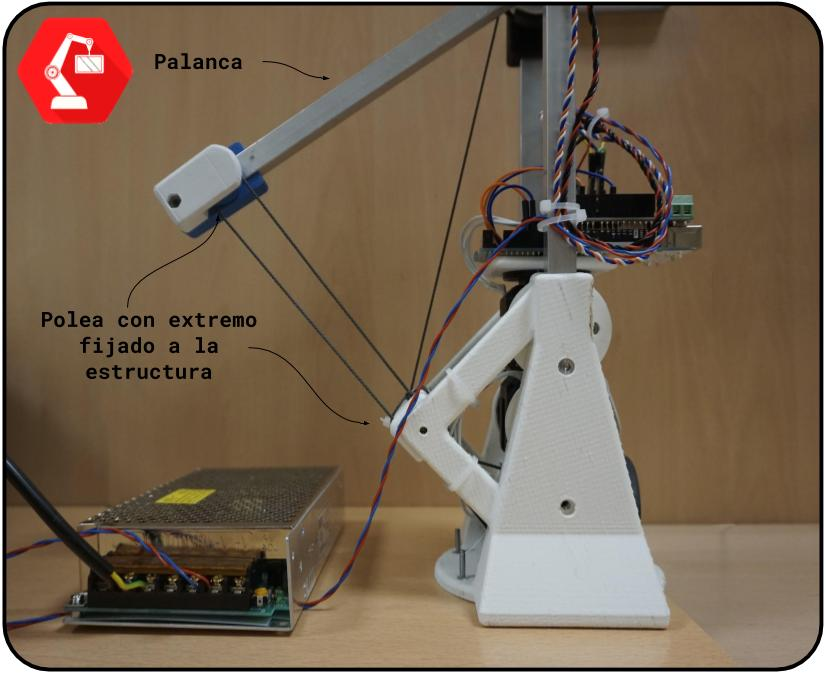
\includegraphics[width=\textwidth]{figuras/Imagenes_Mecanica/foto_brazo_7.jpg}
            \caption{Transmisión hasta la primera articulación}
            \label{fig:Mecanica:columpio_art_uno}
            \immagesource{Autor}
        \end{figure}
    \end{minipage}
    \begin{minipage}{0.56\textwidth}\raggedright
        \begin{figure}[H]
            \centering
            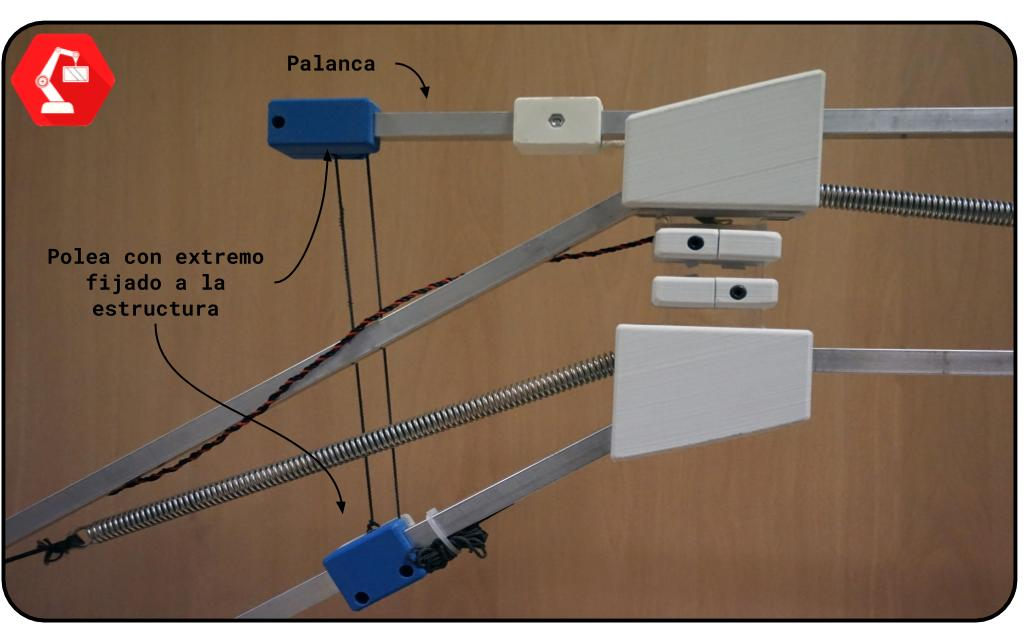
\includegraphics[width=\textwidth]{figuras/Imagenes_Mecanica/foto_brazo_9.jpg}
            \caption{Transmisión del movimiento hasta la segunda articulación}
            \label{fig:Mecanica:columpio_art_dos}
            \immagesource{Autor}
        \end{figure}
    \end{minipage}

    Para conducir los cables de forma controlada hasta los puntos de actuación se ha hecho uso de poleas de redirección, cuyo ensamblaje puede verse en las figuras \ref{fig:Mecanica:redireccion_1} y \ref{fig:Mecanica:redireccion_2}.

    \begin{minipage}{0.47\textwidth}
        \begin{figure}[H]
            \centering
            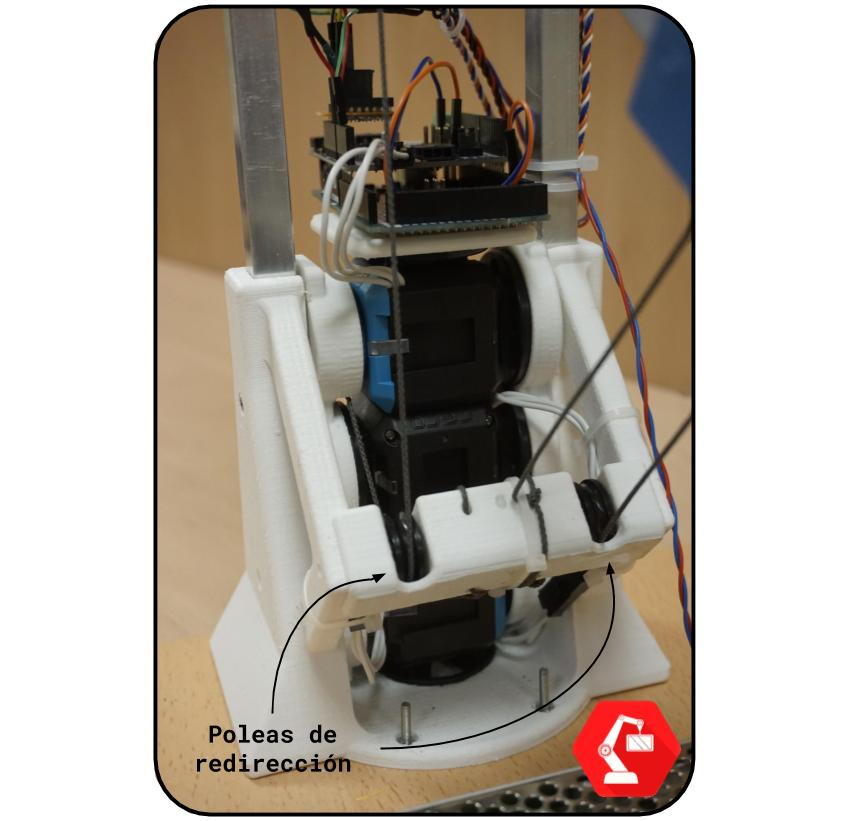
\includegraphics[width=1.15\textwidth]{figuras/Imagenes_Mecanica/foto_brazo_6.jpg}
            \caption{Redirección a la salida de los servomotores}
            \label{fig:Mecanica:redireccion_1}
            \immagesource{Autor}
        \end{figure}
    \end{minipage}
    \begin{minipage}{0.47\textwidth}\raggedright
        \begin{figure}[H]
            \centering
            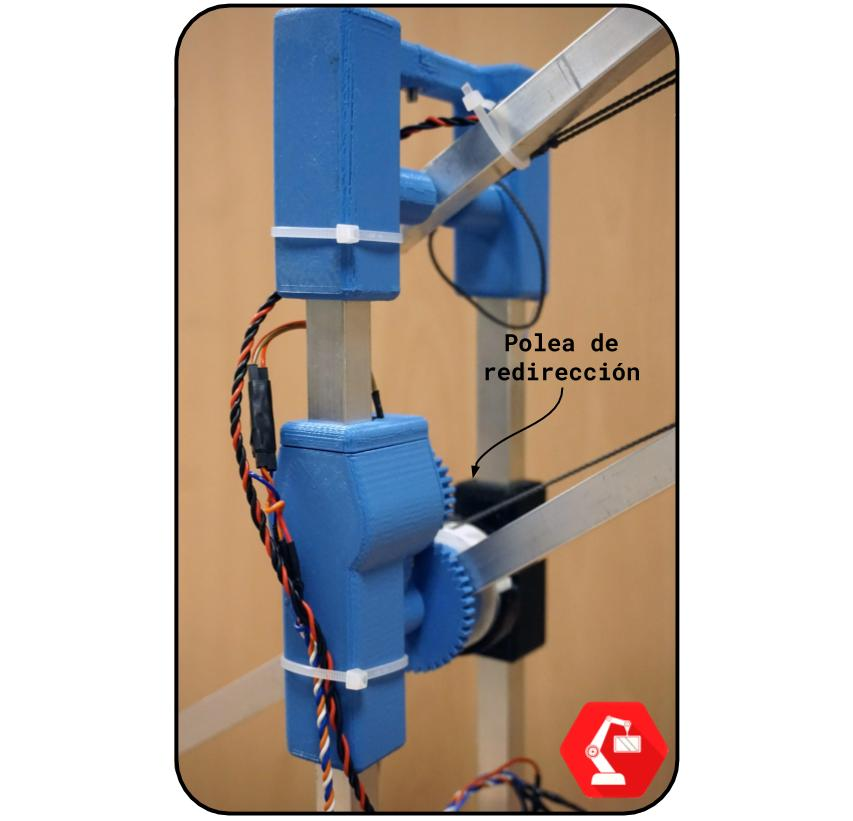
\includegraphics[width=1.15\textwidth]{figuras/Imagenes_Mecanica/foto_brazo_8.jpg}
            \caption{Redirección superior. Eje de la primera articulación}
            \label{fig:Mecanica:redireccion_2}
            \immagesource{Autor}
        \end{figure}
    \end{minipage}

\section{Grados de libertad de la orientación}
\completarCon{¡TBD!}
